\documentclass[sigconf]{acmart}

\usepackage{booktabs} % For formal tables
\usepackage{multirow}
\usepackage[export]{adjustbox}
\usepackage{graphicx}
\usepackage{algorithm}
\usepackage{algorithmic}

% Copyright
%\setcopyright{none}
%\setcopyright{acmcopyright}
%\setcopyright{acmlicensed}
%\setcopyright{rightsretained}
%\setcopyright{usgov}
%\setcopyright{usgovmixed}
%\setcopyright{cagov}
%\setcopyright{cagovmixed}


%% DOI
%\acmDOI{10.475/123_4}

%% ISBN
%\acmISBN{123-4567-24-567/08/06}

%Conference info
%\acmConference[WOODSTOCK'97]{ACM Woodstock conference}{July 1997}{El Paso, Texas USA} 
%\acmYear{1997}
%\copyrightyear{2016}

%\acmPrice{15.00}	


\begin{document}
\title{CMSC 142 MP2: Knight's Tour}



\author{Juancho Meneses}

\email{jrv.meneses@gmail.com}

\author{Gimel Velasco}

\email{gfvelasco@up.edu.ph}



\begin{abstract}
This paper presents an application of a blind search algorithm to the Knight's Tour. For analyzing the performance of the algorithm, the behaviour
of the time it takes to complete a tour starting from 5 different positions is observed.

\end{abstract}



\maketitle

\section{Introduction}
	Considering its flexibility, the knight is the most special piece in chess.  It is the only piece that can jump over other pieces and its movement is not in a straight line which allows it to attack a queen, bishop, or rook without being attacked by that piece in return.  Its move is shaped as an “L” (two squares horizontally or vertically and then one more square perpendicular to the previous direction).\cite{back1} A knight's tour is a sequence of 64 knight moves that visits each square exactly once.\cite{back2} 

	 The objective of this paper is to implement a blind search algorithm of the Knight's tour and analyze the results by recording the time for a solution to be found on different starting positions. The methods used in developing and writing the program and the results obtained from the program will be discussed in the next sections.

\section{Methodology}
	There are many kinds of Blind Search Algorithms or Uninformed Algorithms. Such algorithms are the Depth-First Search (DFS) Algorithm, Breadth-First Search (BFS) Algorithm, Uniform Cost Search (UC), Depth-Limited Search (DL), Iterative Deepening (ID) Search and Bi-directional (BD) Search. For the Knight's Tour Puzzle/Problem, the Depth-First Search is implemented since it is the kind of blind search algorithm that best fits to be able to solve the Knight's Tour Puzzle efficiently even though all of the Uninformed Algorithms will be able to solve the Knight's Tour problem. Compared to the breadth-first approach, the Depth-First approach will be faster in getting a solution since it will go straight into checking a path rather than going through all of the other possible paths. This reason also applies to the Depth-Limited Search and Iterative Deepening Search since there have the same approach like that of a breadth-first search. Now for the Bi-directional Search, the program would be much more complicated to do since it needs to consider the end point of the path--which is not known. But for solving a closed toured Knight's Tour problem, it would be much more useful since the 64th step of the Knight could be easier to predict. So with all the reasons stated above, the Depth-First Search Algorithm is implemented in the problem so that the Knight's Tour puzzle could be solved.\\


	 The pseudo code of the program is shown below.\\
	 
	 \begin{algorithm}
\caption{Pseudo Code of Depth First Backtracking}
\begin{algorithmic} 
\STATE Put Knight in first tile
\WHILE{Knight doesn't have 64 steps}
\STATE Do until there is no more tile to step on
\STATE Jump to the next unvisited tile
\STATE Go back and try the next neighbor
\ENDWHILE
\end{algorithmic}
\end{algorithm}


	The program was created using C programming language.  A snippet of the code of the program is shown in Figure \ref{fig:code}. The rest of the code is also sent together with this paper.
	\begin{figure}[h]
 	 \centering
   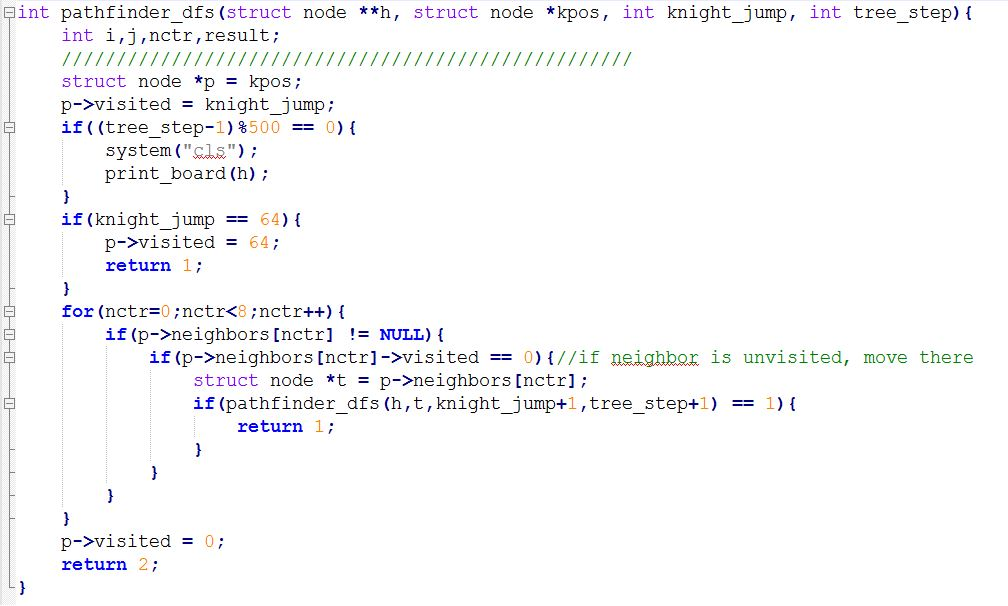
\includegraphics[width=0.5\textwidth]{code.jpg}
  	\caption{Code Snippet}
 	 \label{fig:code}
	\end{figure}
	
	The data structure is given in Figure \ref{fig:datastr}.
	
	\begin{figure}[h]
 	 \centering
   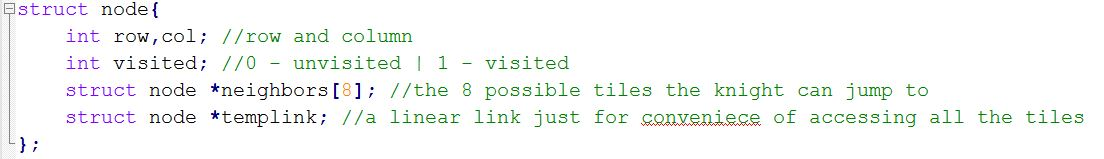
\includegraphics[width=0.5\textwidth]{datastruct.jpg}
  	\caption{Data Structure}
 	 \label{fig:datastr}
	\end{figure}

	The program was run in a Toshiba laptop with Intel(R) Core 2 Duo CPU(2 core(s)) processor, with 4 GB RAM and 64bit operating system.  The program asks for the user to input the starting point of the Knight in the 8x8 board.  The program was run three times in each of the following inputs: A1, A8, H1, H8, and D4.  Other applications such as Google Chrome, Windows Explorer, Spotify, and Sublime Text were also running while the program was being ran.\\
	
\section{Results and Discussions}

	The program outputted the solved board and the completion time of the solution.  The results of the three runs of the different starting positions are can be seen in the following figures.  The running times of the runs of the starting positions is shown in the table below.\\
	
\begin{center}
\begin{tabular}{ |c|c| } 
\hline
Starting Position & Runtime (ms) \\
\hline
\multirow{1}{3em}{A1}
& 20484 \\
\hline
\multirow{1}{3em}{}
& 20597 \\
\hline
\multirow{1}{3em}{}
& 20514 \\
\hline
\multirow{1}{3em}{H1}
& 2251 \\
\hline
\multirow{1}{3em}{}
& 2257 \\
\hline
\multirow{1}{3em}{}
& 2261 \\
\hline
\multirow{1}{3em}{A8}
& 285 \\
\hline
\multirow{1}{3em}{}
& 287 \\
\hline
\multirow{1}{3em}{}
& 286 \\
\hline
\multirow{1}{3em}{H8}
& 741 \\
\hline
\multirow{1}{3em}{}
&  726\\
\hline
\multirow{1}{3em}{}
& 722 \\
\hline
\multirow{1}{3em}{D4}
& 15899629 \\
\hline
\multirow{1}{3em}{}
& 18502156 \\
\hline
\multirow{1}{3em}{}
& 17191270 \\
\hline
\end{tabular}
\end{center}

\begin{figure}[h]
 	 \centering
   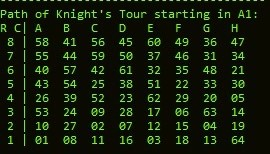
\includegraphics[width=0.5\textwidth]{a1.jpg}
  	\caption{Path from A1}
 	 \label{fig:a1}
	\end{figure}
\begin{figure}[h]
 	 \centering
   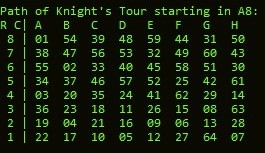
\includegraphics[width=0.5\textwidth]{a8.jpg}
  	\caption{Path from A8}
 	 \label{fig:a8}
	\end{figure}
\begin{figure}[h]
 	 \centering
   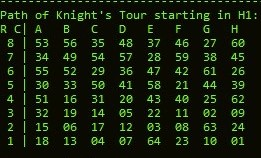
\includegraphics[width=0.5\textwidth]{H1.jpg}
  	\caption{Path from H1}
 	 \label{fig:H1}
	\end{figure}
\begin{figure}[h]
 	 \centering
   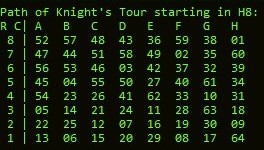
\includegraphics[width=0.5\textwidth]{h8.jpg}
  	\caption{Path from H8}
 	 \label{fig:h8}
	\end{figure}
	\begin{figure}[h]
 	 \centering
   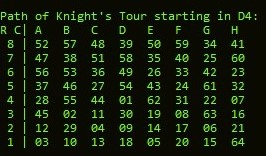
\includegraphics[width=0.5\textwidth]{D41.jpg}
  	\caption{Path from D4}
 	 \label{fig:d4}
	\end{figure}
	Since the program did not randomize in choosing a neighbor position, the path generated by the three runs of a starting position input were the same. As can be observed in the table, starting at the four corners took only few seconds for the knight to complete the tour.  It is reasonable because there are only  two neighbor moves at the corners which means there are only two traversals needed to find a complete 64 jumped positions without repetitions. 
\subsection{Case of Starting Position D4}
	As can be seen in the previous table, starting at the position D4 took a very long time for the knight to complete the tour compared to previous runs starting at the corners.  This is because there are eight neighbor moves in that starting position which also means that it must perform eight traversals of the neighbor moves to find a path which completes the tour. (See similar figure in figure \ref{fig:kpos1})
	\begin{figure}[h]
 	 \centering
   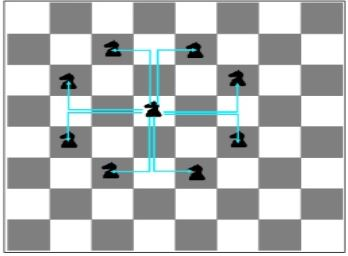
\includegraphics[width=0.5\textwidth]{kpos.jpg}
  	\caption{Similar case of D4 start}
 	 \label{fig:kpos1}
	\end{figure}
	The eight traversals mean that the knight will go to one of the eight neighbor moves at the start and then continuously go to other unvisited neighbor moves until the tour is completed but if starting at that neighbor move did not give a solution, the knight will go back to the starting position which in our case is D4 and it will go to an unvisited neighbor move of the seven remaining neighbor moves at the start and it will go on and on until it finds a solution which completes the tour. 
\section{Conclusions}
Completing the Knight's tour starting from the four corners of an 8x8 board took only few seconds using a blind search algorithm.  Starting at D4 or somewhere at the middle will take long hours to complete the Knight's tour with the use of a blind search algorithm.  The reliability of the algorithm depends on where the starting position is in terms of time complexity. 
%\end{document}  % This is where a 'short' article might terminate






% This next section command marks the start of
% Appendix B, and does not continue the present hierarchy


\bibliographystyle{ACM-Reference-Format}
\nocite{back1}
\bibliography{pres1} 

\end{document}
